
%\chapter*{A brief introduction to quantum field theory in curved spacetimes: Introduction to the Unruh and Hawking effects}[Intro to the Unruh and Hawking effects]
%\label{chap:introUnruh}

\section*{Discussion: Previous results on field entanglement, dimension and statistics}
\markboth{Discussion}{Previous results on field entanglement, dimension and statistics}
\addcontentsline{toc}{chapter}{Discussion: Previous results on field entanglement} 
From the pioneering works that started the analysis of field entanglement behaviour in non-inertial frames it has been shown \cite{Alicefalls,AlsingSchul} that the Unruh effect degrades the entanglement between accelerated partners, affecting all the quantum information tasks that they could perform. 

Fundamental differences were found in these first works between field entanglement of a scalar field \cite{Alicefalls} and a spinless fermionic field (Grassmann scalar) \cite{AlsingSchul}.  Specifically, it was discovered that, as an observer of an entangled state of the field accelerates, entanglement is completely degraded for the scalar case and, conversely, some degree of entanglement survives (even in the limit of infinite acceleration) for the spinless fermionic field\footnote{In literature prior to this thesis only Grassmann scalar fields were considered, this is to say, formal spinless Dirac fields, see Appendix \ref{appB}}.

Let us highlight the main result in \cite{AlsingSchul}. This work presented two observers (Alice and Rob), one of them
inertial and the other one undergoing a constant acceleration $a$. Alice and Rob are the observers of a bipartite quantum state of a spinless fermion field which is maximally entangled for the inertial observer, namely a state of the form
\begin{equation}
\frac{1}{\sqrt{2}}\left(\ket{0_\text{A}0_\text{R}}+\ket{1_\text{A}1_\text{R}}\right).
\end{equation}
As Rob accelerates the Unruh effect
will introduce degradation in the state as seen by Rob, impeding all the
quantum information tasks between both observers.

If we quantify this entanglement by means of negativity $\mathcal{N}$ (see section \ref{entangsec}) following that work\footnote{In \cite{AlsingSchul}  the authors use logarithmic negativity (See \cite{logneg})  instead of negativity. Both entanglement measures are equally valid and are, in fact, very simply related: $L_{\mathcal{N}}=\log_2(2\mathcal N+1)$.} one obtains that the dependence of the negativity with the acceleration gets the simple expression 
\begin{equation}
\mathcal{N}=\frac12\cos^2 r_{\text{f},i},
\end{equation}
where
\begin{equation}
\tan r_{\text{f},i}=\exp(-\pi c{{\omega_i}}/{a}).
\end{equation}
Here $\omega_i$ is the frequency of the mode considered. Notice that in the limit $a\rightarrow\infty$ (which means infinite Unruh temperature), $\mathcal{N}\rightarrow\frac14$, implying that some fermionic entanglement survives the infinite acceleration limit. This was a very unexpected fact, above all taking into account that for the same scenario but considering a bosonic field entanglement is rapidly lost as the accelerated observer increases his acceleration, so that in the limit in which the accelerated observer would observe an infinite Unruh temperature thermal bath\footnote{When observing the inertial vacuum state of the field, see section \ref{tue}.} all entanglement vanishes \cite{Alicefalls}.
 
These previous studies stated that this different behaviour was caused for the difference in the Hilbert space dimension for the different fields. Every different frequency mode for a bosonic field can be excited to an unbounded number of levels, in other words, the dimension of the Fock space for each mode is not bounded. The Fock basis in the fermionic field is, however, limited due to Pauli exclusion principle. For instance, for a spinless fermion field (as the ones considered in these previous works), every frequency is either in the vacuum state or in the excited state, double excitations are forbidden.  For a spin $1/2$ we can have for each frequency one particle or two particles with opposite spin projection quantum numbers, so occupation number is bounded by 2.

As one can intuitively associate the Unruh effect with the observation of thermal noise, it was argued in works prior to this thesis that bosonic fields have a broader margin for the Unruh noise to stochastically excite more levels and degrade entanglement (similar to a decoherence process) while the smaller dimension of the fermionic fields protected them from these random excitations. 

In this first part of the thesis we will study the relationship between field statistics and entanglement behaviour. We will  gain knowledge about the strong relationship between statistics and entanglement degradation step by step. First we will study for the first time spin $1/2$ fermionic fields. This will allow us to study new kinds of entangled states. We will see  that the Dirac field entanglement behaves in exactly the same entanglement degradation that the Grassmann scalar case analysed in previous literature \cite{AlsingSchul}.

Then, by means of a multimode analysis we will prove this behaviour of fermionic fields is universal. Namely, it is independent of  i) the spin of the fermionic field,  ii) the kind of maximally entangled state from which we start, and iii) the dimension of the Fock space of the field for every mode.

We will discover more fundamental differences between fermions and bosons and we will disprove both ways of the statement: fermionic survival is not dependent on dimension and bosonic entanglement disappearance happens even in bosonic settings with a finite dimensional Fock space.

These results together banish the sensible, yet incorrect, argument that linked Fock space dimension with entanglement behaviour in non-inertial frames.

The final chapter of this part I of the thesis will deal with a related but very different topic. The only known work \cite{schacross} previous to this thesis that studies entanglement degradation in the background of a Schwarzschild black hole did not analyse the dependence with the distance to the black hole horizon. Instead the entanglement degradation for observers placed in the asymptotically flat region of spacetime was dealt with.

A more interesting scenario would be to consider observers very close to the event horizon where the gravitational field is strong and the loss of information due to the presence of the horizon is much more intense, so that we can analyse entanglement and correlations as a function of the distance to the horizon.

At the end of this part I, we will rigorously show that tools coming from the constantly accelerated case can be used to study a setting where correlated pairs are shared by observers free-falling into a Schwarzschild black hole and observers resisting the gravitational pull at a finite distance from the event horizon.


\chapter[Spin $1/2$ fields and fermionic entanglement in non-inertial frames]{Spin $1/2$ fields and fermionic entanglement in non-inertial frames\footnote{J. Le\'on, E. Mart\'in-Mart\'inez. Phys. Rev. A, 80, 012314 (2009).}}\label{onehalf}

\markboth{Chapter 3. Spin $1/2$ fields and non-inertial fermionic entanglement}{\rightmark}

%Entanglement behaviour in non-inertial frames was first considered in \cite{Alsingtelep} where the fidelity of teleportation between relative accelerated partners was analysed. After this, occupation number entanglement degradation of scalar \cite{Alicefalls} and Dirac \cite{AlsingSchul} fields due to Unruh effect \cite{Unruh,Crispino} was shown. Recent works studied the effect of the instantaneous Wigner rotations and Thomas spin precession on entanglement \cite{AlsingWigner},\cite{AlsingWignerFot}.


Previous work \cite{AlsingSchul} on Unruh effect for Dirac field mode entanglement does not consider the spin of the parties. This work considered an effective `Grassmann field' where only two occupation numbers $n=(0,1)$ are allowed for each mode. Higher values of $n$ are forbidden by Pauli exclusion principle. However, addressing the effect of Unruh decoherence on spin entanglement can only be done by incorporating the spin of the parties in the framework from the very beginning. As a consequence, occupation number $n=2$ is also allowed. This fact will affect occupation number entanglement which has to be reconsidered in this new setting. For this purpose, we will study here the case of two parties (Alice and Rob) sharing a general superposition of Dirac vacuum and all the possible one particle spin states for both Alice and Rob. Alice is in an inertial frame while Rob undergoes a constant acceleration $a$.

We will show that Rob --when he is accelerated respect to an inertial observer of the Dirac vacuum-- would observe a thermal distribution of fermionic spin $1/2$ particles due to Unruh effect \cite{Unruh}. Next, we will consider that Alice and Rob share spin Bell states in a Minkowski frame. Then, the case in which Alice and Rob share a superposition of the Dirac vacuum and a specific one particle state in a maximally entangled combination. In both cases we analyse the entanglement and mutual information in terms of Rob's acceleration $a$.

Finally, we will study the case when the information about spin is erased from our setting. For this we implement a method to consistently erase such information, keeping only the occupation number information. Here, entanglement is more degraded than in \cite{AlsingSchul} as we are erasing part of the correlations from our system. 

We show that, even in the limit of $a\rightarrow\infty$, some degree of entanglement is preserved due to Pauli exclusion principle. Then we analyse Unruh effect on a completely different class of maximally entangled states (like $\ket{00}+\ket{ss'}$ where $s$ and $s'$ are $z$ component of spin labels) comparing it with the spin Bell states. In section \ref{sec6} we show that the erasure of spin information, in order to investigate occupation number entanglement alone, requires considering total spin states for the bipartite system. 

\section{The setting}\label{sec2}

We consider a free massless Dirac field in a Minkowski frame expanded in terms of the positive (particle) and the negative (antiparticle) energy solutions of Dirac equation in Minkowskian coordinates, denoted $u^+_{\hat\omega,s,\text{M}}$ and $u^-_{\hat\omega,s,\text{M}}$ respectively:
\begin{equation}\label{field}
\phi=\sum_{s}\int d^3k\, (c_{\hat\omega,s,\text{M}}u^+_{\hat\omega,s,\text{M}}+d_{\hat\omega,s,\text{M}}^\dagger u^-_{\hat\omega,s,\text{M}}).
\end{equation}
Here, the subscript $\hat\omega$ denotes Minkowskian frequency and labels the modes of the same energy and $s=\{\uparrow ,\downarrow\}$ is the spin label that indicates spin-up or spin-down along the quantisation axis. $c_{\hat\omega,s,\text{M}}$ and $d_{\hat\omega,s,\text{M}}$ are respectively the annihilation operators for particles and antiparticles, and satisfy the usual anticommutation relations.

For each mode of frequency $\hat\omega$ and spin $s$ the positive and negative energy modes have the form
\begin{equation}\label{eq2}
u^\pm_{\hat\omega,s,\text{M}} =\frac{1}{\sqrt{2\pi \hat\omega}}v^\pm_s(\bm k) e^{\pm i(\bm k\cdot\bm x- \hat\omega t)},\end{equation}
where $v^\pm_s(\hat\omega)$ is a spinor satisfying the usual normalisation relations.

The modes are classified as particle or antiparticle respect to $\partial_t$ (Minkowski Killing vector directed to the future). The Minkowski vacuum state is defined by the tensor product of each frequency mode vacuum
\begin{equation}\label{vacua}\ket0_{\text{M}}=\bigotimes_{\hat\omega}\ket{0_{\hat\omega}}^+_{\text{M}}\ket{0_{\hat\omega}}_{\text{M}}^-\end{equation}
such that it is annihilated by $c_{\hat\omega,s,\text{M}}$ and $d_{\hat\omega,s,\text{M}}$ for all values of $s$.

We will consider the spin structure for each mode, and hence, the maximum occupation number is two. This introduces the following notation
\begin{equation}c^\dagger_{\hat\omega,s,\text{M}}c^\dagger_{\hat\omega,s',\text{M}}\ket0=\ket{ss'_{\hat\omega}}_\text{M}\delta_{s,{-s'}}.\end{equation}
If $s=s'$ the two particles state is not allowed due to Pauli exclusion principle, so our allowed Minkowski states for each mode of particle/antiparticle are
\begin{equation}\{{\ket{0_{\hat\omega}}_\text{M}}^\pm,{\ket{\uparrow_{\hat\omega}}_\text{M}}^\pm,{\ket{\downarrow_{\hat\omega}}_\text{M}}^\pm,{\ket{\pa_{\hat\omega}}_\text{M}}^\pm\},\end{equation}
where $\ket{\pa_{\hat\omega}}^+_\text{M}=c^\dagger_{\hat\omega,\uparrow,\text{M}}c^\dagger_{\hat\omega,\downarrow,\text{M}}\ket{0}_\text{I}$ denotes the spin pair of frequency $\hat\omega$.

To build Rob's field excitations we will work  in the basis \eqref{modopsif} of solutions of the Dirac equation in Minkowski coordinates, whose particularities were explained in section \ref{probexcitations} and such that they correspond to a monochromatic mode when transformed into the Rindler basis. The reason of this is double, on the one hand as we are looking for fundamental behaviour and not the results of a specific experiment there is no reason to adhere to a specific basis, and on the other hand, it is in this basis when we recover the so-called single mode approximation, allowing us to compare our results with previous literature.

Particles and antiparticles will be classified with respect to the future-directed timelike Killing vector in each region. In region I the future-directed Killing vector is
\begin{equation}\label{KillingI}
\partial_\tau^I=\frac{\partial  t}{\partial \tau}\partial_{t}+\frac{\partial x}{\partial \tau}\partial_{x}=a(x\partial_{t}+t\partial_{x}),
\end{equation}
whereas in region II the future-directed Killing vector is $\partial_\tau^{II}=-\partial_\tau^{I}$.

Let us denote $(c_{\omega,s,\text{I}},c^{\dagger}_{\omega,s,\text{I}})$ the particle annihilation and creation operators in region I and $(d_{\omega,s,\text{I}},d^{\dagger}_{\omega,s,\text{I}})$ the corresponding antiparticle operators. Analogously we define $(c_{\omega,s,\text{II}},c^{\dagger}_{\omega,s,\text{II}}, d_{\omega,s,\text{II}},d_{\omega,s,\text{II}}^\dagger)$ the particle/antiparticle operators in region II.

These operators satisfy the usual anticommutation relations $\{c_{\omega,s,\Sigma},c^\dagger_{\omega',s',\Sigma'}\}=\delta_{\Sigma\Sigma'}\delta_{\omega\omega'}\delta_{ss'}$ where the label $\Sigma$ denotes the Rindler region of the operator $\Sigma=\{\text{I},\text{II}\}$. All other anticommutators are zero. That includes the anticommutators between operators in different regions of the Rindler spacetime.

We can relate Minkowskian Unruh modes $\Psi^\text{U}_{\omega,s}$ and Rindler creation and annihilation operators by taking appropriate inner products \cite{Takagi,Jauregui,Birrell,AlsingSchul} as explained in section \ref{probexcitations}. We recall the Bogoliubov coefficients expression \eqref{Bogoferm2}
\begin{eqnarray}\label{Bogoferm3}
\nonumber c_{{\omega_i},\sigma,\text{U}}&=&\cos{r_{\text{d},i}}\,c_{{\omega_i},
\sigma,\text{I}}-\sin r_{\text{d},i}\,d^\dagger_{{\omega_i},-\sigma,\text{II}},\\*
d_{{\omega_i},\sigma,\text{U}}^\dagger&=&\cos{r_{\text{d},i}}\,d^\dagger_{
{\omega_i},\sigma,\text{II}}+\sin r_{\text{d},i}\,c_{{\omega_i},-\sigma,\text{I}},
\end{eqnarray}
and analogously for $c'_{\omega_i}$ and $d'^\dagger_{\omega_i}$ interchanging the labels I and II, where
\begin{equation}\label{defr}
\tan r_{\text{d},i}=\exp(-\pi {c{\omega_i}}/{a}).
\end{equation}

Notice from Bogoliubov transformations \eqref{Bogoferm2} that the Unruh mode particle annihilator $c_{\omega_i,\sigma,\text{U}}$ transforms into a Rindler particle annihilator of frequency $\omega_i$ and spin $s$ in region I and an antiparticle creator of frequency $\omega_i$ and spin $-\sigma$ in region II.


\subsection{Unruh effect for fermion fields of spin $1/2$}\label{sec42m}

Now that we have the relationships between the creation and annihilation operators in the Minkowski and Rindler bases, we can obtain the expression of the Minkowski vacuum state for each mode $\ket{0_{\hat\omega}}_\text{M}$ in the Rindler Fock basis. For notation simplicity, we will drop the $\hat \omega$ and $\omega$ label in operators/states when it does not give any relevant information, but we will continue writing the spin label.

Let us introduce some notation for our states. We will denote with a subscript outside the kets if the mode state is referred to region I or II of the Rindler spacetime. The $\pm$ label of particle/antiparticle will be omitted throughout the chapter because, for the cases considered, a ket referred to Minkowski spacetime or Rindler's region I will always denote particle states and a ket referred to region II will always denote antiparticle states.

Note that here, and in the whole part I of this thesis we will only make use of the `unprimed' particle sector of the Hilbert space in the Minkowskian basis (see section \ref{probexcitations}), this means that Minkowski excitations will always be particles and Rindler excitations will be always particles in the Region I basis and antiparticles in the Region II basis (due to the time reversal anti-symmetry of both regions). From now on and for all this part we drop the label $\pm$ notating particles and antiparticles in the kets. The complete analysis of the antiparticle sector behaviour is dealt with in section \ref{secferme}.

Inside the ket we will write the spin state of the modes as follows
\begin{equation}\label{notation1}
\ket{s}_\text{I}=c^\dagger_{s,\text{I}}\ket{0}_\text{I},\qquad \ket{s}_{\text{II}}=d^\dagger_{s,\text{II}}\ket{0}_{\text{II}},
\end{equation}
which will denote a particle state in region I and an antiparticle state in region II respectively, both with spin $s$.

We will use the following definitions for the kets associated to particle pairs
\begin{eqnarray}\label{notation2}
\nonumber \ket{\pa}_\text{I}&=&c^\dagger_{\uparrow\text{I}}c^\dagger_{\downarrow\text{I}}\ket{0}_\text{I}=-c^\dagger_{\downarrow\text{I}}c^\dagger_{\uparrow\text{I}}\ket{0}_\text{I},\\*
\ket{\pa}_\text{II}&=&d^\dagger_{\uparrow\text{II}}d^\dagger_{\downarrow\text{II}}\ket{0}_\text{II}=-d^\dagger_{\downarrow\text{II}}d^\dagger_{\uparrow\text{II}}\ket{0}_\text{II},
\end{eqnarray}
and, being consistent with the anticommutation relations for different Rindler wedges,
\begin{equation}\label{notation3}
\nonumber \ket{s}_\text{I}\ket{s'}_\text{II}=c^\dagger_{s,\text{I}}d^\dagger_{s',\text{II}}\ket{0}_{I}\ket{0}_\text{II}=-d^\dagger_{s',\text{II}}c^\dagger_{s,\text{I}}\ket{0}_{I}\ket{0}_\text{II},
\end{equation}
\begin{equation}\label{notation4}
d^\dagger_{s',\text{II}}\biket{s}{0}=-\biket{s}{s'}.
\end{equation}

The Bogoliubov transformation \eqref{Bogoferm2} is a fermionic two-modes squeezing transformation for each $\omega_i$, indeed
\begin{equation}\label{upinthesky}\left(\!\begin{array}{c}
c_{\omega_i,s,\text{U}}\\
d^\dagger_{\omega_i,s,\text{U}}
\end{array}\!\right)=S\left(\!\begin{array}{c}
c_{\omega_i,s,\text{I}}\\
d^\dagger_{\omega_i,-s,\text{II}}
\end{array}\!\right)S^\dagger,\end{equation}
where
\begin{equation}\label{squeez}
S=\exp\left[r\left(c_{\omega_i,s,\text{I}}^\dagger\, d_{\omega_i,-s,\text{II}}+c_{\omega_i,s,\text{I}}\, d_{\omega_i,-s,\text{II}}^\dagger \right)\right].
\end{equation}
Note that, for notational convenience given the length and complexity of the expressions, we will drop the labels $\omega_i$ and d from $r$ when the distinction between different frequencies and fermions and bosons is not required to be explicitly shown.

Now, given \eqref{upinthesky} and analogously to \cite{Alicefalls,AlsingSchul}, it is reasonable to postulate that for every $\omega_i$ the Minkowski vacuum is a Rindler two-mode particles/antiparticles squeezed state with opposite spin and momentum states in I and II.

Considering that the modes have spin, occupation number is allowed to be 2 for each frequency, being higher occupation numbers forbidden by Pauli exclusion principle. We need to compute the coefficients of the squeezed state\footnote{One must be careful with the tensor product structure of the fermionic vacuum. Here we present only the `unprimed sector' of the vacuum state. While this is simpler and perfectly valid for the particular choice of inertial Unruh modes presented here, the whole vacuum must be considered in more general scenarios when we consider modes that combine `primed' and `unprimed' Unruh modes. This fact and its consequences are thoroughly analysed in section \ref{secferme}.}
\begin{equation}\label{vacuum0}
 \ket{0}=V\biket{0}{0}+A\biket{\uparrow}{\downarrow}+B\biket{\downarrow}{\uparrow}+ C\biket{\pa}{\pa}.
\end{equation}

To obtain the values of the coefficients $V,A,B,C$ we demand that the Minkowski vacuum is annihilated by the particle annihilator, $c_{\hat\omega, s,\text{M}}\ket0=0$ for all frequencies. As Unruh modes are purely positive frequency combination of Minkowskian modes, this is equivalent to demand that the vacuum is annihilated by all the particle annihilators of Unruh modes \eqref{modopsi}: $c_{\omega, s,\text{U}}\ket0=0$. Translating this into the Rindler basis we have
\begin{equation}\label{annihil2}
\left[\cos r\,c_{s,\text{I}}-\sin r\,d^\dagger_{-s,\text{II}}\right]\left[V\biket{0}{0}+A\biket{\uparrow}{\downarrow}+B\biket{\downarrow}{\uparrow}+ C\biket{\pa}{\pa}\right]=0.
\end{equation}
This equation gives 4 conditions (two for each value of $s$), although only 3 of them are independent:
\begin{equation}
\left.\begin{array}{lcr}
A\cos r - V\sin r&=&0\\
C\cos r - B\sin r&=&0\\
B\cos r - V\sin r&=&0\\
C\cos r - A\sin r&=&0\\
\end{array}\right\}\Rightarrow \begin{array}{ll}A=B=V \tan r\\
C=V\tan^2 r
\end{array}.
\end{equation}
To fix $V$ we impose the normalisation relation for each field mode $\braket{0}{0}=1\Rightarrow |V|^2=1-|A|^2-|B|^2-|C|^2$, this yields the values of the vacuum coefficients:
\begin{equation}\label{vaccoef}
\begin{array}{lcl}
V&=&\cos^2 r,\\
A&=&\sin r\,\cos r, \\
B&=&\sin r\,\cos r,\\
C&=&\sin^2 r.\\
\end{array}
\end{equation}

So, finally, the Minkowski vacuum state in the Rindler basis reads as follows
\begin{equation}\label{vacuum}
 \ket{0}=\cos^2 r\,\biket{0}{0}+\sin r\,\cos r\left(\biket{\uparrow}{\downarrow}+\biket{\downarrow}{\uparrow}\right)+\sin^2 r\,\biket{\pa}{\pa},
\end{equation}
where, to simplify notation, we drop the label M for the Minkowski vacuum which is annihilated by both Unruh and monochromatic Minkowskian modes particle and antiparticle annihilators.

Now we have to know how the excited states (of spin $s$) look like in the Rindler basis. This can be readily obtained by applying the Unruh particle creation operator to the vacuum state $\ket{s}_\text{U}=c^\dagger_{s,\text{U}}\ket0$, and translating it into the Rindler basis:
\begin{align}\label{onepart1}
 \nonumber\ket{s}_\text{U}&=\left[\cos r c^\dagger_{s,\text{I}}-\sin r d_{-s,\text{II}}\right]\left[\cos^2 r\biket{0}{0}+\sin r\cos r\left(\biket{\uparrow}{\downarrow}+\biket{\downarrow}{\uparrow}\right)\right.\\*
 &\left.+\sin^2 r\biket{\pa}{\pa}\right],
\end{align}
which gives
\begin{eqnarray}\label{onepart2a}
\nonumber\ket\uparrow_\text{U}&=&\cos r \biket{\uparrow}{0}+e^{i\phi}\sin r\biket{\pa}{\uparrow},\\*
\ket\downarrow_\text{U}&=&\cos r \biket{\downarrow}{0}-e^{i\phi}\sin r\biket{\pa}{\downarrow}.
\end{eqnarray}

Now, since Rob is experiencing a uniform acceleration, he will not be able to access to field modes in the causally disconnected region II, hence, Rob must trace over that unobservable region. Specifically, when Rob is in region I of Rindler spacetime and Alice observes the vacuum state, Rob can only observe a non-pure partial state given by $\rho_\text{R}=\tr_\text{II}\left(\ket{0}\bra{0}\right)$, which yields
\begin{equation}\label{partialvacuum}
\rho_\text{R}=\cos^4 r\ket{0}_\text{I}\!\!\bra{0}+\sin^2 r\,\cos^2 r\left(\ket{\uparrow}_\text{I}\!\!\bra{\uparrow}+\ket{\downarrow}_\text{I}\!\!\bra{\downarrow}\right)+\sin^4 r \ket{\pa}_\text{I}\!\bra{\pa}.
\end{equation}
Thus, while Alice would observe the vacuum state of mode $k$, Rob would observe a certain statistical distribution of particles. The expected value of Rob's number operator on the Minkowski vacuum state is given by
\begin{equation}
\langle N_\text{R}\rangle=\ematriz{0}{N_\text{R}}{0}=\tr_{I,II}\left(N_\text{R}\proj{0}{0}\right)=\tr_{I}\left(N_\text{R}\rho_\text{R}\right)=\tr_{I}\left[\left(c_{\uparrow\text{I}}^\dagger c_{\uparrow\text{I}}+c_{\downarrow\text{I}}^\dagger c_{\downarrow\text{I}}\right)\rho_\text{R}\right].
\end{equation}
Substituting the expression \eqref{partialvacuum} we obtain
\begin{equation}
\langle N_\text{R}\rangle=2\sin^2 r,
\end{equation}
which, using \eqref{defr}, reads 
\begin{equation}\label{Unruh}
\langle N \rangle=2\frac{1}{e^{2\pi\omega c/a}+1}=2\frac{1}{e^{\hslash\omega/K_BT}+1},
\end{equation}
where $k_B$ is the Boltzmann's constant and
\begin{equation}
T=\frac{\hslash\, a}{2\pi k_B c},
\end{equation}
is the Unruh temperature.

Equation \eqref{Unruh} is an alternative derivation of the well known Unruh effect \cite{DaviesUnr,Unruh} for a fermionic field. We have shown that an uniformly accelerated observer in region I detects a thermal Fermi-Dirac distribution when he observes the Minkowski vacuum. The factor 2 appears due to the degeneracy factor $2S+1$.

\section{Spin entanglement with an accelerated partner}\label{sec5}

In previous works \cite{Alicefalls,AlsingSchul} it was studied how Unruh decoherence affects occupation number entanglement in bipartite states of the type\footnote{Since Alice is an inertial observer, it is not relevant if Alice's excitations are monochromatic or `unprimed' Unruh modes. In either case all the results are exactly the same. To keep the notation as simple as possible we will label Alice's mode with the label `U' used for Unruh modes in this Part I of the thesis. See chapter \ref{sma} for further details.}
\begin{equation}\label{alsingst}
\ket{\Psi}=\frac{1}{\sqrt2}(\ket{0}\ket{0}+\ket{1}_\text{U}\ket{1}_\text{U})
\end{equation}of a  Grassmann scalar field, barring any reference to the spin of the field modes. The figures inside the kets represent occupation number of Alice and Rob modes respectively.

Here, where we have included the spin structure of each mode in our setting from the very beginning, it is possible to study the effects of acceleration in spin entanglement degradation, which is different from the mere occupation number entanglement.

Specifically, with this setting we are able to study how acceleration affects the entanglement of spin Bell states when Alice and Rob share a maximally entangled spin state and Rob accelerates. In the Minkowski basis, these 4 maximally entangled states take the form
\begin{equation}\label{Bellstates}\ket\psi^\pm=\frac{1}{\sqrt2}\left[\ket{\uparrow_\text{A}}_\text{U}\ket{\downarrow_\text{R}}_\text{U}\pm\ket{\downarrow_\text{A}}_\text{U},\ket{\uparrow_\text{R}}_\text{U}\right]\qquad\ket\phi^\pm=\frac{1}{\sqrt2}\left[\ket{\uparrow_\text{A}}_\text{U}\ket{\uparrow_\text{R}}_\text{U}\pm\ket{\downarrow_\text{A}}_\text{U},\ket{\downarrow_\text{R}}_\text{U}\right].\end{equation}

First of all, we build a general bipartite state that could be somehow analogous to state \eqref{alsingst} studied in \cite{AlsingSchul}. This state will be a superposition of the vacuum and all the possible 1-particle bipartite states for Alice and Rob.
\begin{equation}\label{genstate}
\ket{\Psi}=\mu\ket{0}\ket{0}+\alpha\ket{\uparrow}_\text{U}\ket{\uparrow}_\text{U}+\beta\ket{\uparrow}_\text{U}\ket{\downarrow}_\text{U}+ \gamma\ket{\downarrow}_\text{U}\ket{\uparrow}_\text{U}+\delta\ket{\downarrow}_\text{U}\ket{\downarrow}_\text{U},
\end{equation}
with $\mu=\sqrt{1-|\alpha|^2-|\beta|^2-|\gamma|^2-|\delta|^2}$.

This state generalises the Bell spin states (for instance, we have $\ket{\phi^+}$ choosing $\alpha=\delta=1/\sqrt2$) or a occupation number entangled state (for instance choosing $\alpha=\mu=1/\sqrt2$).  We will be able to deal with two different and interesting problems: 1. Studying the Unruh effect on  spin entangled states and 2. Investigating the impact of considering the spin structure of the fermion on the occupation number entanglement and its Unruh entanglement degradation.

The density matrix in the Minkowskian Unruh basis for the state \eqref{genstate} is
\begin{align}\label{Minkowdens}
\nonumber\rho^M&=\mu^2\proj{00}{00}+\mu\alpha^*\proj{00}{\uparrow\uparrow}+\mu\beta^*\proj{00}{\uparrow\downarrow}+\mu\gamma^*\proj{00}{\downarrow\uparrow}+\mu\delta^*\proj{00}{\downarrow\downarrow}\\*
\nonumber &+|\alpha|^2\proj{\uparrow\uparrow}{\uparrow\uparrow}+\alpha\beta^*\proj{\uparrow\uparrow}{\uparrow\downarrow}+\alpha\gamma^*\proj{\uparrow\uparrow}{\downarrow\uparrow}+\alpha\delta^*\proj{\uparrow\uparrow}{\downarrow\downarrow}+|\beta|^2\proj{\uparrow\downarrow}{\uparrow\downarrow}\\*
&+\beta\gamma^*\proj{\uparrow\downarrow}{\downarrow\uparrow}\!+\!\beta\delta^*\proj{\uparrow\downarrow}{\downarrow\downarrow}\!+\!|\gamma|^2\proj{\downarrow\uparrow}{\downarrow\uparrow}\!+\!\gamma\delta^*\proj{\downarrow\uparrow}{\downarrow\downarrow}\!+\!|\delta|^2\proj{\downarrow\downarrow}{\downarrow\downarrow}\!+\! (\text{H.c.})_{_{\substack{\text{non-}\\\text{diag.}}}},
\end{align}
where $(\text{H.c.})_{\text{non-diag.}}$ means non-diagonal Hermitian conjugate, and represents the Hermitian conjugate only for the non-diagonal elements.

Again, as Rob can only carry out measurements in his accessible Fock basis (made of only region I modes) we need to compute each term of \eqref{Minkowdens} in the Rindler basis and trace over the unobserved region II.

Computing the density matrix, taking into account that Rob is constrained to region I of Rindler spacetime, requires to rewrite Rob's mode in the Rindler basis and to trace over the unobservable Rindler's region II. It is useful to compute first the trace over II on all the operators that compose \eqref{Minkowdens}. Using equation \eqref{vacuum} we have
\begin{equation}
\proj{00}{00}\!=\!\ket{0_\text{A}}\left[\cos^2 r\biket{0}{0}\!+\!\sin r\cos r \left(\biket{\uparrow}{\downarrow}\!+\!\biket{\downarrow}{\uparrow}\right)\!+\!\sin^2 r\biket{\pa}{\pa}\right]\otimes \text{H.c.},
\end{equation}
where the label A indicates Alice's subsystem. Tracing over II:
\begin{equation}\label{trazapa1}
\tr_\text{II}\proj{00}{00}=\cos^4 r\proj{00}{00}+\sin^2r\,\cos^2r\left(\proj{0\uparrow}{0\uparrow}+\proj{0\downarrow}{0\downarrow}\right)+\sin^4r\proj{0\pa}{0\pa},
\end{equation}
where notation is different in each side of the equality: bras and kets in l.h.s. are in the Minkowskian basis $\ket{ss'}=\ket{s_\text{U}}\ket{s'_\text{U}}$ and in the r.h.s. they are referred to Alice's mode in the Minkowskian basis and Rob's mode in the Rindler's region I Fock basis $\ket{ss'}=\ket{s_\text{U}}\ket{s'_\text{R}}_\text{I}$.

In the same way, using expressions \eqref{vacuum}, \eqref{onepart2a} we have
\begin{align}
\nonumber\proj{00}{ss'}=&\ket{0_\text{A}}\left[\cos^2 r\,\biket{0}{0}+\sin r\,\cos r\left(\biket{\uparrow}{\downarrow}+\biket{\downarrow}{\uparrow}\right)+\sin^2 r\biket{\pa}{\pa}\right]\\*&\bra{s_\text{A}}\left(\cos r\,{\bra{s'}_\text{I}}\,{\bra{0}_\text{II}}+ \varepsilon\, \sin r\,{\bra{\pa}_\text{I}}\,{\bra{s'}_\text{II}}\right),
\end{align}
where $\varepsilon=1$ if $s=\uparrow$ and $\varepsilon=-1$ if $s=\downarrow$. Now, tracing over II
\begin{equation}\label{trazapa2}
\tr_\text{II}\proj{00}{ss'}=\cos^3 r\,\proj{00}{ss'}+\sin^2r\,\cos r\left(\delta_{s'\uparrow}\proj{0\downarrow}{s\pa}-\delta_{s'\downarrow}\proj{0\uparrow}{s\pa}\right),
\end{equation}
with the same notation used in \eqref{trazapa1}.

Similarly, using expression \eqref{onepart2a} we get
\begin{align}
\nonumber\proj{s_1s_2}{s_3s_4}&=\ket{{s_{1}}_\text{A}}\left[\cos r\,\biket{s_2}{0}+\varepsilon_2e^{-i\phi}\sin r\biket{\pa}{s_2}\right]\bra{{s_{3}}_\text{A}}\left[\cos r\,{\bra{s_4}_\text{I}}{\bra{0}_\text{II}}\right.\\*
&\left.+\,\varepsilon_4\sin r\,{\bra{\pa}_\text{I}}{\bra{s_4}_\text{II}}\right],
\end{align}
and tracing over II gives
\begin{equation}\label{trazapa3}
\tr_\text{II}\proj{s_1s_2}{s_3s_4}=\cos^2 r\,\proj{s_1s_2}{s_3s_4}+\delta_{s_2s_4}\sin^2r\proj{s_1\pa}{s_3\pa}.\\*
\end{equation}
Again, notation here is the same than in \eqref{trazapa1}.

 Using \eqref{trazapa1}, \eqref{trazapa2}, \eqref{trazapa3} we can easily compute the density matrix for Alice and Rob from \eqref{Minkowdens} since $\rho_{AR}=\tr_\text{II}\rho_M$, resulting in the long expression
\begin{align}\label{generaldensmat}
\nonumber\rho_{AR}&\!=\!\mu^2\Big[\!\cos^4r\proj{00}{00}\!+\!\sin^2r\cos^2r\left(\proj{0\!\uparrow}{0\!\uparrow}\!+\!\proj{0\!\downarrow}{0\!\downarrow}\right)\!+\!\sin^4r\proj{0\pa}{0\pa}\!\Big]\!+\!\mu\cos^3\!r\\*
\nonumber&\times\Big[\alpha^*\proj{00}{\uparrow\uparrow}\!+\!\beta^*\proj{00}{\uparrow\downarrow}\!+\!\gamma^*\proj{00}{\downarrow\uparrow}\!+\!\delta^*\proj{00}{\downarrow\downarrow}\Big]\!+\!\mu\sin^2r\cos r\Big[\alpha^*\proj{0\downarrow}{\uparrow\pa}\\*
\nonumber&-\beta^*\!\proj{0\!\uparrow}{\uparrow\!\pa}\!+\!\gamma^*\!\proj{0\!\downarrow}{\downarrow\!\pa}\!-\!\delta^*\!\proj{0\!\uparrow}{\downarrow\!\pa}\Big]\!+\!\cos^2 r\Big[|\alpha|^2\proj{\uparrow\uparrow}{\uparrow\uparrow}\!+\!\alpha\beta^*\proj{\uparrow\uparrow}{\uparrow\downarrow}\!+\!\alpha\gamma^*\\*
\nonumber&\times\proj{\uparrow\uparrow}{\downarrow\uparrow}\!+\!\alpha\delta^*\proj{\uparrow\uparrow}{\downarrow\downarrow}\!+\!|\beta|^2\proj{\uparrow\downarrow}{\uparrow\downarrow}\!+\!\beta\gamma^*\proj{\uparrow\downarrow}{\downarrow\uparrow}\!+\!\beta\delta^*\proj{\uparrow\downarrow}{\downarrow\downarrow}\!+\!|\gamma|^2\proj{\downarrow\uparrow}{\downarrow\uparrow}\\*
\nonumber&+\gamma\delta^*\proj{\downarrow\uparrow}{\downarrow\downarrow}+|\delta|^2\proj{\downarrow\downarrow}{\downarrow\downarrow}\Big]+\sin^2r\Big[\left(|\alpha|^2+|\beta|^2\right)\proj{\uparrow\pa}{\uparrow\pa}+\left(|\gamma|^2+|\delta|^2\right)\\*
&\times\proj{\downarrow\pa}{\downarrow\pa}+\left(\alpha\gamma^*+\beta\delta^*\right)\proj{\uparrow\pa}{\downarrow\pa}\Big]+(\text{H.c.})_{_{\substack{\text{non-}\\\text{diag.}}}}.
\end{align}
Here the notation is the same than in the r.h.s. of \eqref{trazapa1}. We see that the state, which in the Minkowski basis is pure, becomes mixed when the observer Rob is accelerated due to the causal disconnection of the accelerated observer with part of the spacetime.


Equation \eqref{generaldensmat} will be our starting point, from which we will study different entanglement settings and how Unruh effect affects them.

We will now compute how acceleration affects the entanglement of spin Bell states \eqref{Bellstates} when Alice and Rob share a maximally entangled spin state and Rob accelerates. A specific choice of coefficients in \eqref{genstate} gives us these states, namely
\begin{align}
\ket{\phi^\pm}\Rightarrow \alpha=\pm\delta=\frac{1}{\sqrt{2}},\\*
\ket{\psi^\pm}\Rightarrow \beta=\pm\gamma=\frac{1}{\sqrt{2}},
\end{align}
and all the other coefficients equal to zero. For such states in the Minkowski basis, the density matrix of Alice and Rob when he undergoes an acceleration $a$ is obtained from \eqref{generaldensmat}:
\begin{equation}\label{Phibell}
\rho^{\phi^\pm}_{AR}\!=\!\frac12\Big[\cos^2 r\Big(\proj{\uparrow\uparrow}{\uparrow\uparrow}\pm\proj{\uparrow\uparrow}{\downarrow\downarrow}\pm\proj{\downarrow\downarrow}{\uparrow\uparrow}\!+\!\proj{\downarrow\downarrow}{\downarrow\downarrow}\Big)+\sin^2 r\Big(\!\proj{\uparrow\!\pa}{\uparrow\!\pa}+\proj{\downarrow\!\pa}{\downarrow\!\pa}\!\Big)\Big],
\end{equation}
\begin{equation}\label{Psibell}
\rho^{\psi^\pm}_{AR}\!=\!\frac12\Big[\cos^2 r\Big(\proj{\uparrow\downarrow}{\uparrow\downarrow}\pm\proj{\uparrow\downarrow}{\downarrow\uparrow}\pm\proj{\downarrow\uparrow}{\uparrow\downarrow}\!+\!\proj{\downarrow\uparrow}{\downarrow\uparrow}\Big)+\sin^2 r\Big(\!\proj{\uparrow\!\pa}{\uparrow\!\pa}+\proj{\downarrow\!\pa}{\downarrow\!\pa}\!\Big)\Big].
\end{equation}

Notice that, in this case, Rob has a qutrit, since for his mode he could have three different possible orthogonal states: particle spin-up, particle spin-down and particle pair. This is an important difference with the spinless case: the Hilbert space dimension of the accelerated observer increases when he is accelerating, what was a qubit in the Minkowskian basis is now a qutrit in the Rindler basis for Rob.

To characterise its entanglement we will use the negativity \eqref{negativitydef}. To compute it we need the partial transpose density matrices (defined in \eqref{ptranspdef}) of the states \eqref{Phibell} and \eqref{Psibell}
\begin{equation}
\rho^{\phi^\pm pT}_{AR}\!\!\!=\!\frac12\Big[\cos^2 r\Big(\proj{\uparrow\uparrow}{\uparrow\uparrow}\pm\proj{\uparrow\downarrow}{\downarrow\uparrow}\pm\proj{\downarrow\uparrow}{\uparrow\downarrow}\!+\!\proj{\downarrow\downarrow}{\downarrow\downarrow}\Big)+\sin^2 r\Big(\!\proj{\uparrow\!\pa}{\uparrow\!\pa}+\proj{\downarrow\!\pa}{\downarrow\!\pa}\!\Big)\Big],
\end{equation}
\begin{equation}
\rho^{\psi^\pm pT}_{AR}\!\!\!=\!\frac12\Big[\cos^2 r\Big(\proj{\uparrow\downarrow}{\uparrow\downarrow}\pm\proj{\uparrow\uparrow}{\downarrow\downarrow}\pm\proj{\downarrow\downarrow}{\uparrow\uparrow}\!+\!\proj{\downarrow\uparrow}{\downarrow\uparrow}\Big)+\sin^2 r\Big(\!\proj{\uparrow\!\pa}{\uparrow\!\pa}+\proj{\downarrow\!\pa}{\downarrow\!\pa}\!\Big)\Big].
\end{equation}
We can write $\rho^{\phi^\pm pT}_{AR}$ matricially in the basis $\left\{\ket{\uparrow\uparrow},\ket{\uparrow\downarrow},\ket{\downarrow\uparrow},\ket{\downarrow\downarrow},\ket{\uparrow\pa},\ket{\downarrow\pa}\right\}$ and $\rho^{\psi^\pm pT}_{AR}$ in the basis $\left\{\ket{\uparrow\downarrow},\ket{\uparrow\uparrow},\ket{\downarrow\downarrow},\ket{\downarrow\uparrow},\ket{\uparrow\pa},\ket{\downarrow\pa}\right\}$. Both have the same expression
\begin{equation}
\frac12\left(\!\begin{array}{cccccc}
\cos^2 r & 0 &0 &0 & 0 & 0\\
0&0 &\pm\cos^2 r &0 & 0 & 0 \\
0  &\pm\cos^2 r  &0 &0 &0 &0 \\
0  & 0 &0 &\cos^2 r &0 &0 \\
0 & 0 &0&0& \sin^2 r &0 \\
0& 0& 0&0&0& \sin^2 r \\
\end{array}\!\right).
\end{equation}
Therefore the four Bell states will have the same eigenvalues. The only negative eigenvalue is
\begin{equation}
\lambda_-=-\frac12\cos^2r.
\end{equation}

Since $r=\arctan\left(e^{-\pi\frac{\omega c}{a}}\right)$ $a\rightarrow0\Rightarrow r\rightarrow 0$ and $a\rightarrow\infty\Rightarrow r\rightarrow \pi/4$ so that $\lambda_6$ is negative for all values of the acceleration. This implies, using Peres criterion \cite{PeresCriterion}, that the spin Bell states will be always entangled even in the limit of infinite acceleration.

We can readily evaluate the entanglement at the limits $a\rightarrow0$ and $a\rightarrow\infty$ if we compute the negativity for these states, which have the trivial form
\begin{equation}
\mathcal{N}(r)=\frac12\cos^2 r.
\end{equation}
In the limit $a\rightarrow0$ we obtain $\mathcal{N}=\dfrac12$ which is an expected result since $a\rightarrow0$ is the inertial limit.

However, in the limit $a\rightarrow\infty$ we obtain $\mathcal{N}=\frac{1}{4}$, which implies that spin entanglement degrades due to the Unruh effect up to a certain limit.

In \cite{AlsingSchul} it is discussed (for occupation number entangled states of a spinless fermion field) that Pauli exclusion principle protects the occupation number entanglement from degrading, and some degree of entanglement is preserved even at the limit $a\rightarrow\infty$. The striking result is that here we have obtained a mathematically identical result for the spin Bell states. We will discuss later how this result, along with many others presented in this thesis, will disprove the statement that the finite dimension of the Fock space is responsible for this entanglement survival in the $a\rightarrow\infty$ limit.

\section{Vacuum and 1-particle entangled superpositions}

Next, we will study the case in which Alice and Rob share a different class of maximally entangled state, we consider that in the Minkowski Unruh basis we have
\begin{equation}\label{minkstate2}
\ket{\Psi}=\frac{1}{\sqrt2}\left(\ket{0_\text{A}}\ket{0_\text{R}}+\ket{\uparrow_\text{A}}_\text{U}\ket{\downarrow_\text{R}}_\text{U}\right),
\end{equation}
which is a maximally entangled state that includes occupation number entanglement along with spin. We study this kind of states as a first analog to the state considered in previous literature \eqref{alsingst}. This state corresponds to the choice
\begin{align}\label{coef22}
\beta&=\mu=\frac{1}{\sqrt2},\\*
\alpha&=\gamma=\delta=0
\end{align}
in equation \eqref{generaldensmat}. The density matrix of such a state is
\begin{align}\label{minkstate2R}
\nonumber\rho&=\frac12\Big[\cos^4r\proj{00}{00}+\sin^2r\cos^2r\left(\proj{0\!\uparrow}{0\!\uparrow}+\proj{0\!\downarrow}{0\!\downarrow}\right)+\sin^4r\proj{0\pa}{0\pa}\\*
&+\cos^3r\left(\proj{00}{\uparrow\downarrow}+\proj{\uparrow\downarrow}{00}\right)-\sin^2r\cos r\left(\proj{0\!\uparrow}{\uparrow\!\pa}+\proj{\uparrow\!\pa}{0\!\uparrow}\right)+\cos^2r\proj{\uparrow\downarrow}{\uparrow\downarrow}\nonumber\\*
&+\sin^2r\proj{\uparrow\!\pa}{\uparrow\!\pa}\Big].
\end{align}
Notice the significant difference from the Bell spin states; considering that Rob accelerates means that, this time, Alice has a qubit and Rob has a four dimensional quantum system. Since in Rindler coordinates the state \eqref{minkstate2R} is qualitatively very different from the Minkowski Bell states \eqref{Phibell}, \eqref{Psibell}, it is therefore worthwhile to study its entanglement degradation as Rob accelerates.

The partial transpose of \eqref{minkstate2R} is
\begin{align}\label{minkstate2R2}
\nonumber\rho^{pT}&=\frac12\Big[\cos^4r\proj{00}{00}+\sin^2r\cos^2r\left(\proj{0\uparrow}{0\uparrow}+\proj{0\downarrow}{0\downarrow}\right)+\sin^4r\proj{0\pa}{0\pa}\\*
\nonumber&+\cos^3r\left(\proj{0\!\downarrow}{\uparrow\!0}+\proj{\uparrow\!0}{0\!\downarrow}\right)-\sin^2r\,\cos r\left(\proj{0\pa}{\uparrow\uparrow}+\proj{\uparrow\uparrow}{0\pa}\right)\!+\!\cos^2r\proj{\uparrow\downarrow}{\uparrow\downarrow}\\*
&+\sin^2r\proj{\uparrow\!\pa}{\uparrow\!\pa}\Big],
\end{align}
which is a $8\times8$ block-diagonal matrix. It has two non-positive eigenvalues
\begin{align}\label{eig2}
\nonumber\lambda_{1}&=\frac{1}{4}\left(\sin^2r\cos^2r-\sqrt{\sin^4r\cos^4r+4\cos^6r}\right)\\*
\lambda_{2}&=\frac14\left(\sin^4r-\sqrt{\sin^8r+4\sin^4r\,\cos^2r}\right).
\end{align}
As we can see, $\lambda_2$ is non-positive and $\lambda_1$ is negative for all values of $a$, therefore the state will always preserve some degree of distillable entanglement. If we calculate the negativity we will obtain
\begin{equation}
\mathcal{N}(r)=\frac12\cos^2r,
\end{equation}
which means that for this case, distillable entanglement behaves exactly as in the previous case. In other words, no matter if the entangled state is a spin Bell state or a superposition like \eqref{minkstate2}, entanglement degrades the same. To conclude this section we stress that the same results will be obtained if the state $\ket{\uparrow_\text{A}}_\text{U}\ket{\downarrow_\text{A}}_\text{U}$ in \eqref{minkstate2} is replaced by any other 1 particle bipartite spin state $\ket{ss'}_\text{U}$.

\section{Non-inertial occupation number entanglement for spin $1/2$ fermions}\label{sec6}

The previous work \cite{AlsingSchul} on occupation number entanglement between accelerated partners ignored the spin structure of the Dirac field modes. It is not possible to straightforwardly translate a state like \eqref{genstate} into mere occupation number states. This comes about because for a state like \eqref{genstate} the bipartite vacuum component does not have individual spin degrees of freedom as the other components do. In other words, by including the vacuum state in the superposition \eqref{genstate}, the Hilbert space ceases to be factorable in terms of individual spin times particle occupation number subspaces.

On the other hand, the bipartite vacuum is a well defined total spin singlet. Hence, the Hilbert space is factorable with respect to the total spin of the system A-R and the occupation number subspaces. Accordingly, to reduce the spin information in the general density matrix \eqref{generaldensmat} we will be forced to consider a factorisation of the Hilbert space as the product of the total spin and occupation number subspaces.

Taking this tensor product structure into account we can now formally consider that we are not able to access to the information of the total spin of the system $A-R$ and then, we should trace over total spin degree of freedom.

The equivalence between the standard basis (occupation number-individual spin) and the new basis (occupation number-total spin) is\footnote{The pair state in the same mode can only be a singlet of total spin due to anticommutation relations of fermionic fields.}
\begin{equation}\label{e1}
\begin{array}{cc}
\ket{00}=\ket{00}\ket{S}& \ket{0\pa}=\ket{02}\ket{S},\\*[1.5mm]
\ket{0\uparrow}=\ket{01}\ket{D_+}& \ket{0,\downarrow}=\ket{01}\ket{D_-},\\*[1.5mm]
\ket{\uparrow0}=\ket{10}\ket{D_+}&\ket{\downarrow0}=\ket{10}\ket{D_-},\\*[1.5mm]
\ket{\uparrow\pa}=\ket{12}\ket{D_+}&\ket{\downarrow\pa}=\ket{12}\ket{D_-},\\*[1.5mm]
\ket{\uparrow\uparrow}=\ket{11}\ket{T_+}&\ket{\downarrow\downarrow}=\ket{11}\ket{T_-},\\*[1.5mm]
\end{array}
\end{equation}
\begin{equation}\label{e2}
\begin{array}{c}
\ket{\uparrow\downarrow}=\frac{1}{\sqrt{2}}\ket{11}\left[\ket{T_0}+\ket{S}\right],\\*[1.5mm]
\ket{\downarrow\uparrow}=\frac{1}{\sqrt{2}}\ket{11}\left[\ket{T_0}-\ket{S}\right],
\end{array}
\end{equation}
where we are using the basis $\ket{n_\text{A}\,n_\text{R}}\ket{J,J_z}$ and the triplets, doublets and the singlet are denoted as
\begin{eqnarray}
\nonumber\ket{T_+}&=&\ket{J=1,J_z=1},\\*
\nonumber\ket{T_-}&=&\ket{J=1,J_z=-1},\\*
\nonumber\ket{T_0}&=&\ket{J=1,J_z=0},\\*
\nonumber\ket{D_+}&=&\ket{J=1/2,J_z=1/2},\\*
\nonumber\ket{D_-}&=&\ket{J=1/2,J_z=-1/2},\\*
\nonumber\ket{S}&=&\ket{J=0,J_z=0}.\\*
\end{eqnarray}
Rewriting the general state \eqref{genstate} in this basis we obtain
\begin{equation}\label{genstateb2}
\ket{\Psi}=\mu\ket{00}\ket{S}+\alpha\ket{11}\ket{T_+}+\frac{\beta+\gamma}{\sqrt2}\ket{11}\ket{T_0}+ \frac{\beta-\gamma}{\sqrt2}\ket{11}\ket{S}+\delta\ket{11}\ket{T_-}
\end{equation}
Considering the acceleration of Rob, the general state \eqref{generaldensmat} in terms of this new basis after reducing the information on the total spin by tracing over this degree of freedom is
\begin{equation}
\rho^n_{AR}=\sum_{J,J_z}\bra{J,J_z}\rho_{AR}\ket{J,J_z}.
\end{equation}
Which results in a state in the occupation number basis whose entanglement degradation incorporates the effect of the spin structure. This can be studied and compared with the results in reference \cite{AlsingSchul} in which spin existence is ignored.
\begin{align}\label{densityred}
\nonumber\rho^n_{AR}&=\mu^2\Big[\cos^4r\proj{00}{00}+2\sin^2r\,\cos^2r\proj{01}{01}+\sin^4r\proj{02}{02}\Big]+\mu\cos^3r\\*
&\!\!\times\left(\frac{\beta^*-\gamma^*}{\sqrt2}\proj{00}{11}\!+\!\frac{\beta-\gamma}{\sqrt2}\proj{11}{00}\right)\!+\!(1-\mu^2)\Big[\cos^2r\proj{11}{11}\!+\!\sin^2r\proj{12}{12}\Big].
\end{align}
We can readily compute the partial transpose 
\begin{align}\label{densityred}
\nonumber(\rho^n_{AR})^{pT}&=\mu^2\Big[\cos^4r\proj{00}{00}+2\sin^2r\,\cos^2r\proj{01}{01}+\sin^4r\proj{02}{02}\Big]+\mu\cos^3r\\*
&\!\!\!\!\!\!\!\!\!\!\!\!\!\!\!\times\left(\frac{\beta^*-\gamma^*}{\sqrt2}\proj{01}{10}+\frac{\beta-\gamma}{\sqrt2}\proj{10}{01}\right)\!+\!(1-\mu^2)\Big[\cos^2r\proj{11}{11}\!+\!\sin^2r\proj{12}{12}\Big],
\end{align}
which only has a negative egigenvalue. The negativity is, in this case,
\begin{equation}\label{negativitymode}
\mathcal{N}=\cos^2r\left|\mu^2\sin^2r-\mu\sqrt{\mu^2\sin^4r+\cos^2r\frac{|\beta-\gamma|^2}{2}}\right|,
\end{equation}
which depends on the proportion of singlet \mbox{$|\beta-\gamma|/\sqrt2$} of the $\ket{11}$ component in the state \eqref{genstate}. When there is no singlet component ($\beta=\gamma$) the negativity is zero. Indeed in the limit $a\rightarrow0$ (Minkowskian limit)
\begin{equation}\label{negativitymode0}
\mathcal{N}_0=\frac{1}{\sqrt2}\left|\mu\right|\left|\beta-\gamma\right|,
\end{equation}
which shows that the maximally entangled Minkowski occupation number state (Negativity $=1/2$) arises tracing over total spin when the starting state is
\begin{equation}\label{modesmaxen}
\ket{\Psi}=\frac{1}{\sqrt2}\ket{00}\pm\frac12\big[\ket{\uparrow\downarrow}-\ket{\downarrow\uparrow}\big],
\end{equation}
or, in the occupation number-total spin basis
\begin{equation}\label{modesmaxen2}
\ket{\Psi}=\frac{1}{\sqrt2}\Big[\ket{00}\ket{S}\pm\ket{11}\ket{S}\big].
\end{equation}
This means that, for occupation number entanglement, the only way to have an entangled state of the bipartite vacuum $\ket{00}$ and the one particle state $\ket{11}$ of a Dirac field is through the singlet component of total spin for the $\ket{11}$ component.

On the contrary, the state
\begin{equation}
\ket{\Psi}=\frac{1}{\sqrt2}\Big[\ket{00}\ket{S}\pm\ket{11}\ket{T_{0,\pm}}\big]
\end{equation}
will become separable after tracing over total spin due to the orthonormality of the basis \eqref{e1}, \eqref{e2}.

We have established that the Minkowski maximally entangled state for occupation number arises after tracing over total spin in a state as \eqref{modesmaxen}. Now we will compute the limit of the negativity when the acceleration goes to $\infty$ in order to see its Unruh decoherence and to compare it with the results for occupation number entanglement from \cite{AlsingSchul}.

Taking $a\rightarrow\infty \Rightarrow r\rightarrow\pi/4$ in \eqref{negativitymode}
\begin{equation}\label{negativitymodeinfty}
\mathcal{N}_\infty=\frac14\left|\mu^2-\sqrt{\mu^4+\mu^2|\beta-\gamma|^2}\right|.
\end{equation}
Therefore, for the maximally Minkowski entangled state we have $\mu=1/\sqrt{2}$, $|\beta-\gamma|=1$ and the negativity in the limit is
\begin{equation}\label{negalimi}
\mathcal{N}_\infty=\frac{\sqrt3-1}{8}.
\end{equation}

\begin{figure}[H]
\begin{center}
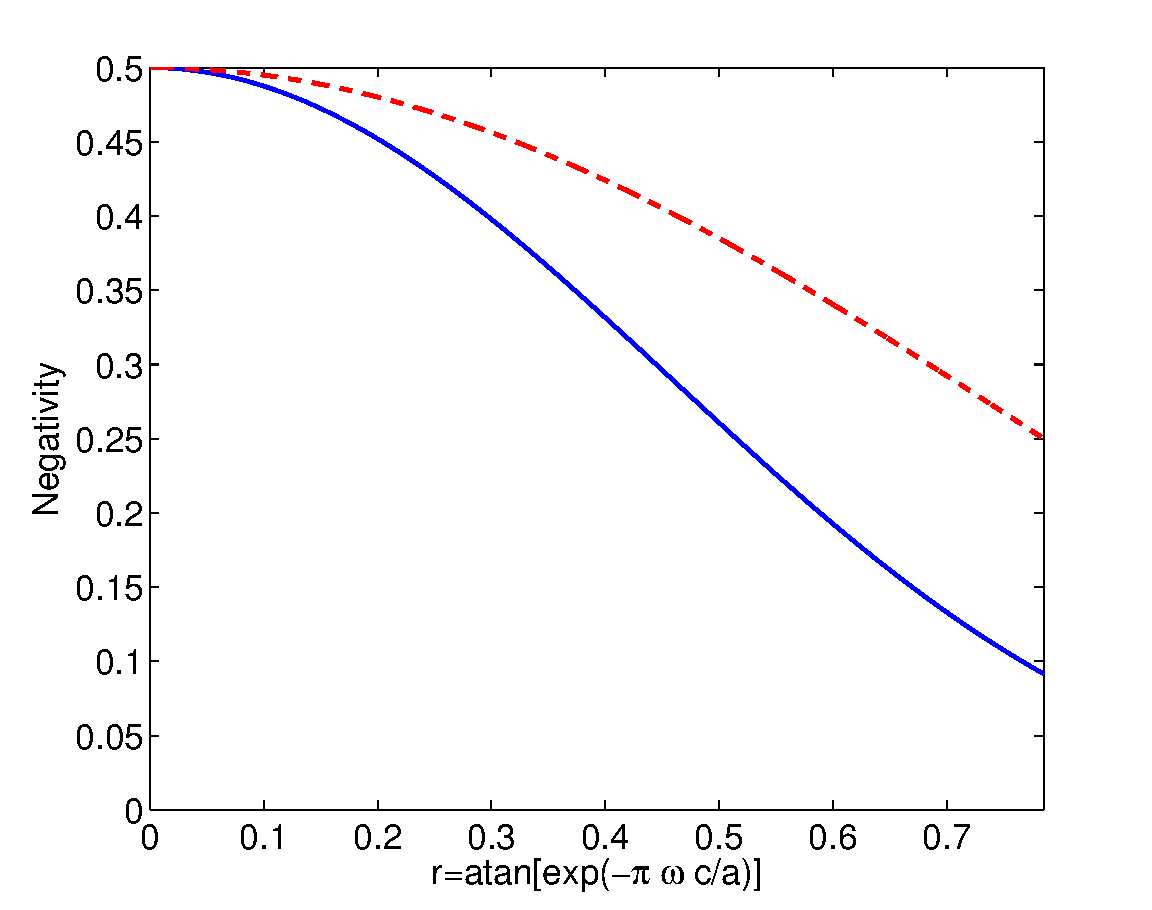
\includegraphics[width=.85\textwidth]{mutumode}
\end{center}
\caption{(Blue solid) Negativity in the occupation number degree of freedom as a function of the acceleration of Rob when A and R share an occupation number maximally entangled state \eqref{modesmaxen} in the Minkowski basis after tracing over total spin. (Red dashed) Negativity a as a function of the acceleration of Rob when A and R share spin Bell states and the state $\frac{1}{\sqrt2}\left(\ket{00}+\ket{ss'}\right)$ (both cases coincide).}
\label{fig5}
\end{figure}

This result shows that when we reduce the total spin information, looking at the occupation number entanglement alone, we see that it is more degraded by the Unruh effect than when we considered spin Bell states in the previous section. More importantly, the occupation number entanglement is more degraded than in \cite{AlsingSchul}, where the spin structure of the modes was considered nonexistent. This happens because we are removing part of the correlations when we erase total spin information. The negativity dependence on the acceleration is shown in Fig. \ref{fig5} compared with the negativity for the maximally entangled states \eqref{Bellstates} and \eqref{minkstate2}.




\section{Discussion}\label{sec7}

It is known \cite{Alicefalls,AlsingSchul} that Unruh decoherence degrades entanglement of occupation number states of fields. Here we have shown a richer casuistic that appears when we take into account that each Dirac mode has spin structure. This fact enables us to study interesting effects (such as entanglement degradation for spin Bell states) and develop new procedures to erase spin information from the system in order to study occupation number entanglement.

Along this chapter we have analysed how a maximally entangled spin Bell state losses entanglement when one of the partners accelerates. We have seen that, while in the Minkowski basis Alice and Rob have qubits, when Rob accelerates the system becomes a non-pure state of a qubit for Alice and a qutrit for Rob. In this case spin entanglement for a Dirac field is degraded when Rob accelerates. However some degree of entanglement survives even at the limit $a\rightarrow\infty$.

A first difference with previous literature where spin was not taken into account is that in this case the dimension of the Hilbert space changes when we consider the state in Rob's Fock basis. A first analog to the well studied state $(1/\sqrt{2})(\ket{00}+\ket{11})$ but including spin, $(1/\sqrt{2})(\ket{00}+\ket{\uparrow\downarrow})$, has been studied. This state,  becomes $2\times 4$ dimensional when Rob accelerates. On the other hand,  Spin Bell states becomes a $2\times3$  dimension system. Nevertheless, we have demonstrated distillable entanglement degrades exactly in the same way as for spin Bell states and for other maximally entangled superposition. This fact will be deeply analysed in following chapters.

The Fock space for every mode of a Dirac field has higher dimension than for the spinless fermionic field as the one analysed in \cite{AlsingSchul} (the basis for every mode changes from $\ket{0},\ket{1}$ to $\{\ket{0},\ket{\uparrow},\ket{\downarrow},\ket{\pa}$). Indeed, we have seen how for a Dirac field, the dimension of the Hilbert space is increased when Rob accelerates due to the excitation of spin pairs.

 However, we have seen that in spite of the evident differences between the spinless fermionic field analysed in the literature and the spin $1/2$ field analysed here, the entanglement degradation due to the Unruh effect is exactly the same in both cases. More striking: even spin Bell states (which had no analog in a Grassmann scalar field) have the same entanglement behaviour as the states described above. This starts to suggest some sort of universal behaviour present in fermionic fields. This is a first argument against  the idea that the Hilbert space dimension is connected with the entanglement survival in the infinite acceleration limit for fermions. We will explore this in the following chapters. 

We have also introduced a procedure to consistently erase spin information from our setting preserving the occupation number information. We have done it by tracing over total spin. The maximally entangled occupation number state is obtained from the total spin singlet \eqref{modesmaxen} after tracing over total spin. Finally we have shown that its entanglement is more degraded than in \cite{AlsingSchul} where the spin structure of Dirac modes was neglected. 


\cleardoublepage
